\documentclass[12pt,parskip=full, tikz]{article}

% Packages
\usepackage{amsmath}
\usepackage{graphicx}
\usepackage{hyperref}
\usepackage{float}
\usepackage{geometry}
\geometry{a4paper, margin=1in}
\usepackage{tikz}
\usetikzlibrary{positioning, arrows.meta, fit} % Load the positioning library
\usetikzlibrary{patterns}
\usepackage{amsmath}
\usepackage{amsthm}
\usepackage{caption}
\usepackage{subcaption}
\usepackage[parfill]{parskip}
\usepackage{cleveref}
\usepackage{listings}

\newtheorem{theorem}{\textsf{Theorem}}
\newtheorem{corollary}[theorem]{\textsf{Corollary}}
\newtheorem{definition}[theorem]{\textsf{Definition}}
\newtheorem{assumption}[theorem]{\textsf{Assumption}}
\newtheorem{lemma}[theorem]{\textsf{\textsf{Lemma}}}
\newtheorem{claim}[theorem]{\textsf{\textsf{Claim}}}
\newtheorem{proposition}[theorem]{\textsf{Proposition}}



\setlength{\parindent}{0pt}
\setlength{\parskip}{0.8em}

% Document begins
\begin{document}

% Title
\title{Decentralized Farming Contracts}
\author{MuesliSwap Team}
\date{\today}
\maketitle

% Abstract
\begin{abstract} \noindent
This document proposes and outlines the design and implementation plan for a new decentralized staking and farming system within the Cardano ecosystem. Addressing the limitations of existing partially decentralized solutions, the proposed system ensures that every aspect, including reward computation, is managed entirely on-chain, thereby achieving maximum decentralization. By focusing on a fully on-chain operation, this approach enhances trustlessness and transparency. Additionally, the document includes a comparative analysis of current solutions across various blockchain platforms, which serves as motivation for the design choices and highlights the benefits of the proposed system.
\end{abstract}
\newpage 

% Table of Contents
\tableofcontents
\newpage

\section*{Executive Summary}
This section will provide a brief overview of the research findings and the proposed decentralized staking system.

\section{Introduction}

\subsection{Background}

In the realm of Decentralized Finance (DeFi), staking and farming play a crucial role by providing incentives that encourage user participation and liquidity provision. The advent of smart contracts offers a unique opportunity to execute these processes in a trustless manner, eliminating the need for intermediaries. Setting such incentives has been a key aspect and driver in the success of DeFi as a whole. 

As part of the Cardano Catalyst Funding program, this document delves into the next step of advancing and further decentralizing staking and farming solutions on Cardano. It achieves this by comparing existing solutions on Cardano and other blockchain platforms and proposing a novel architecture. This proposal spans from high-level concepts to detailed technical implementation on Cardano.

\subsection{Problem Statement}

Current solutions are often only partially decentralized. While locking mechanisms are typically implemented via smart contracts, the mechanisms for distributing rewards and ensuring sufficient rewards are provided are frequently managed by centralized services that require user trust. 

On the road towards a fully decentralized, DAO-based DeFi platform, there is a need for a completely decentralized staking and farming solution. Such a solution should be fully implemented in smart contracts, with reward funds controlled via community governance and reward payouts guaranteed by the contracts themselves. This would enable users to trustlessly rely on a platform that is entirely self-governed.

\subsection{Purpose of the Document}

This document serves as a detailed guide to understanding existing solutions, their respective design choices, opportunities, and limitations. It aims to identify properties that are most desirable in a fully decentralized staking and farming system. The document proposes an architecture for a robust framework satisfying these requirements, presented initially as an overview and sketch, followed by concrete implementation details in the form of Cardano smart contracts interacting with each other. 

The document is intended for developers, technically interested users, and decision-makers in the DeFi space, particularly on Cardano.

\paragraph{Scope} The scope of this document encompasses four main points:
\begin{enumerate}
    \item A design overview and detailed architecture of individual components, as well as a description of their interplay.
    \item Implementation details for both on-chain and off-chain components, including security measures taken to ensure the safety of the smart contract design.
    \item A comparative analysis of existing on-chain and off-chain staking and farming models, highlighting their strengths, weaknesses, and applicability in various contexts.
    \item An outline of a comprehensive implementation plan, including development phases, timeline, and milestones envisioned along the way.
\end{enumerate}
The goal is to ensure an efficient implementation of the project, guided by thorough understanding and high security and quality standards.


\section{System Design and Architecture}

\subsection{Overview of Decentralized Staking System}

\subsubsection{Objectives}

The fundamental concept of staking revolves around locking, or depositing, a specific amount of token A into a smart contract for a predetermined duration. Once this period elapses, the tokens can be unlocked, with the smart contract ensuring that only the wallet which initially locked the position can perform the unlocking. As a reward for this action, users receive a certain amount of other tokens, such as B, C, etc. The reward amount depends on various factors: the duration of the lock, the amount locked, and potentially the number of other active staking positions at the same time. This mechanism provides a trustless and automated way to incentivize token holders to participate in the protocol's security and functionality.

Farming, on the other hand, builds upon the staking mechanism by specifically incentivizing the locking of LP (liquidity provider) tokens. These tokens are typically obtained by providing liquidity to decentralized exchanges or other liquidity pools. Farming thus aims to further incentivize liquidity provision within the ecosystem. In a truly decentralized system, the community can actively direct liquidity flows by adjusting rewards through a governance process. This allows for dynamic and responsive management of liquidity incentives, ensuring the system remains robust and efficient.

\subsubsection{Design Principles}

\paragraph{Decentralization}

Decentralization is the cornerstone of this project, alongside security. The aim is to eliminate reliance on any centralized entity throughout the entire process. This means no single entity should have the power to halt the protocol, alter reward emission schedules, or influence reward payouts. Every aspect of the system must be controllable via community-driven governance mechanisms. This principle ensures that the protocol remains resilient, censorship-resistant, and aligned with the broader goals of decentralizing finance. It also fosters a more inclusive environment where all stakeholders have a voice in the protocol's evolution and management.

\paragraph{Security}

Security in DeFi protocols is paramount due to the significant value often locked within these systems. This project places a strong emphasis on safeguarding these assets, encompassing locked funds, funds reserved for future reward payouts, and the rewards themselves. The design must ensure that these assets are protected against a range of threats, including hacks, exploits, and manipulations. Additionally, the protocol must be secure against the risk of centralization, where a single entity or a small group could manipulate the system. By prioritizing security, we aim to build a system that users can trust, thus fostering wider adoption and long-term sustainability.

\paragraph{Transparency}

Transparency is another critical design principle. All interactions with the protocol should be publicly visible and easily understandable as transactions on the Cardano blockchain. This visibility allows users to verify reward payouts, observe reserved reward funds, and generally audit the system to ensure fairness and integrity. Transparency fosters trust among participants, as they can independently confirm that the protocol operates as intended. It also enhances accountability, as any deviations or malfunctions can be quickly identified and addressed by the community.

\paragraph{Modularity}

The system is designed to be modular, consisting of a suite of smart contracts rather than a single monolithic contract. This modularity is intentional, allowing different components to be independently upgraded, replaced, or extended. Such a design ensures that the protocol can adapt to new technologies, user needs, and regulatory environments. Modular design also facilitates easier debugging, testing, and verification of individual components, enhancing the overall robustness and security of the system. Future improvements can be integrated seamlessly, guided by community governance.

\paragraph{Upgradeability and Flexibility}

Finally, the protocol's components must be upgradeable through an on-chain governance process. This ensures that the system remains flexible and can evolve over time in response to the rapidly changing DeFi landscape. Upgradeability is crucial for maintaining decentralization, security, transparency, and modularity in the long term. It allows the community to introduce new features, improve existing functionalities, and address emerging challenges without compromising the protocol's core principles. This adaptability is essential for staying competitive and ensuring the protocol continues to meet user needs effectively.


\subsubsection{Architecture}
On a high level, the system consists of a) a contract at which the locked UTxO represent the available farms/staking pools which maintain some basic parameters, as well as data for keeping track of the currently staked amount, b) a set of contract facilitating the staking itself (i.e. UTxOs containing the user's staked funds), and c) another contract managing the reward allocation to farms based on their rank in the list of highest-volume liquidity pools.

In practice, item b), i.e.\ the farms contract, will be integrated into one of the contracts from item a), since having two separate contracts would create circular dependencies of the form: contract A needs to know contract B's address and vice versa.

\subsection{Details on Components and Interactions}

Next, we elaborate in more detail on the involved components by giving an overview on how each of the following parts are implemented.

\subsubsection{Staking Contracts}
The staking system consists of a so-called \emph{Batching} contract, as well as a \emph{Staking Positions} contract. The former is used to place an ``order'' expressing the intent to open a staking position. A (decentralized) batching bot can then spend this request UTxO and is forced by the \emph{Batching} contract to open a staking position with correctly initialized datum information by creating a UTxO at the \emph{Staking Position} contract with respective datum. An authentication NFT must necessarily be minted when creating creating staking positions, s.t.\ its minting script can check the validity of the created position (otherwise everyone could create UTxOs with arbitrary datum at the \emph{Staking Position} contract). Similarly, for unstaking, a respective ``order'' is placed at the \emph{Batching} contract. In order for the batching bot to unlock a staking position on the owner's behalf, an unstake permission NFT is included in the order that is valid for a specific staking position.

\subsubsection{Governance-Based Farms}
In order to support creation of farms by anyone and with reward token funds coming from various sources, while guaranteeing that sufficient reward funds are always available for paying out stakers/farmers, we use a \emph{Farms} contract. In practice this contract will coincide with the \emph{Staking Positions} contract, as otherwise we get a circular dependencies on these contracts' addresses. The \emph{Farms} contract ensures that a sufficient amount of reward tokens are locked at the UTxO representing a specific farm, i.e., sufficient to pay out rewards up to a certain validity date (publicly known to stakers/farmers). The \emph{Farms} contract is oblivious to where funds used to initialize the farm are coming from. Hence anyone can open a farm, given that they provide sufficient reward tokens. In particular, this enables farm initialization via a payout tally from the MuesliSwap onchain governance system.

\subsubsection{Top-Pools Contracts}
In addition to governance-controlled farms, we want to support farms with reward payouts based on the performance/popularity of the respective liquidity pools (in terms of the pool's total value locked (TVL)). For this, a separate contract, the so-called \emph{Top-Pools} contract is necessary. This contract maintains a list of liquidity pool identifiers, ordered by TVL. Items in the list can be re-arranged in case TVLs change by providing the repspective pool UTxOs a reference inputs to the modifying transaction. Reward funds are allocated according to the rank of a farm in the \emph{Top-Pools} list.


\section{Implementation \& Further Technical Details}

Next, we provide further technical details. This is done by schematically illustrating the transactions involved in a farm creation and staking workflow. Below, we give a detailed description and diagram of various of the involved steps.

\subsection{Placing \& Cancelling Stake Orders}

\begin{figure}
    \centering
    \begin{subfigure}[b]{0.45\textwidth}
        \centering
        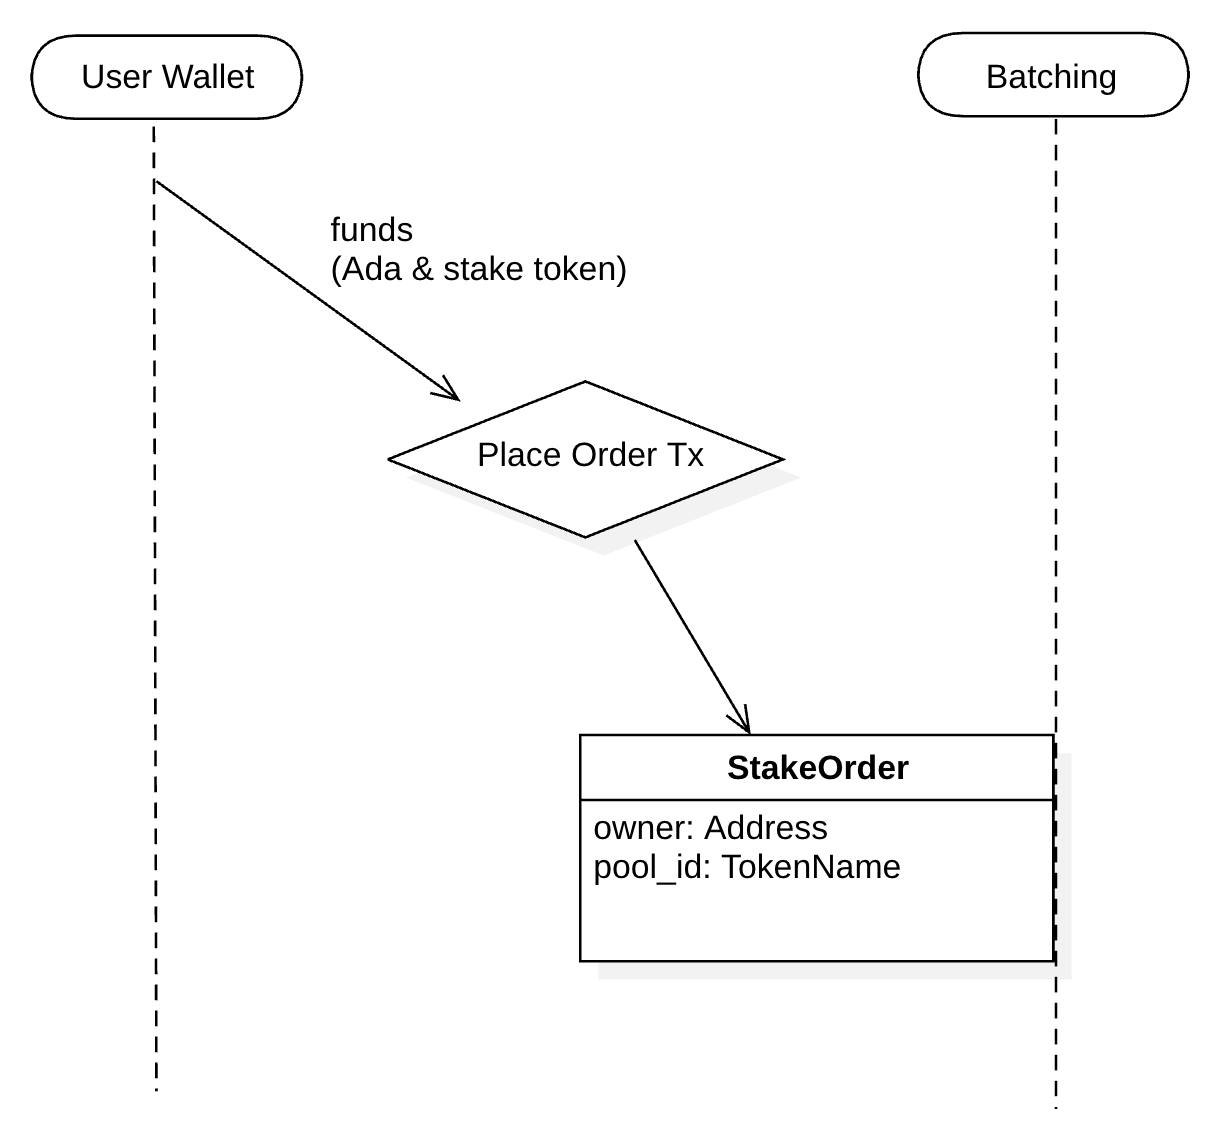
\includegraphics[width=\textwidth]{figures/place-stake-order.png}
        \caption{Placing a stake order.}
        \label{fig:place-stake-order}
    \end{subfigure}
    \hfill
    \begin{subfigure}[b]{0.45\textwidth}
        \centering
        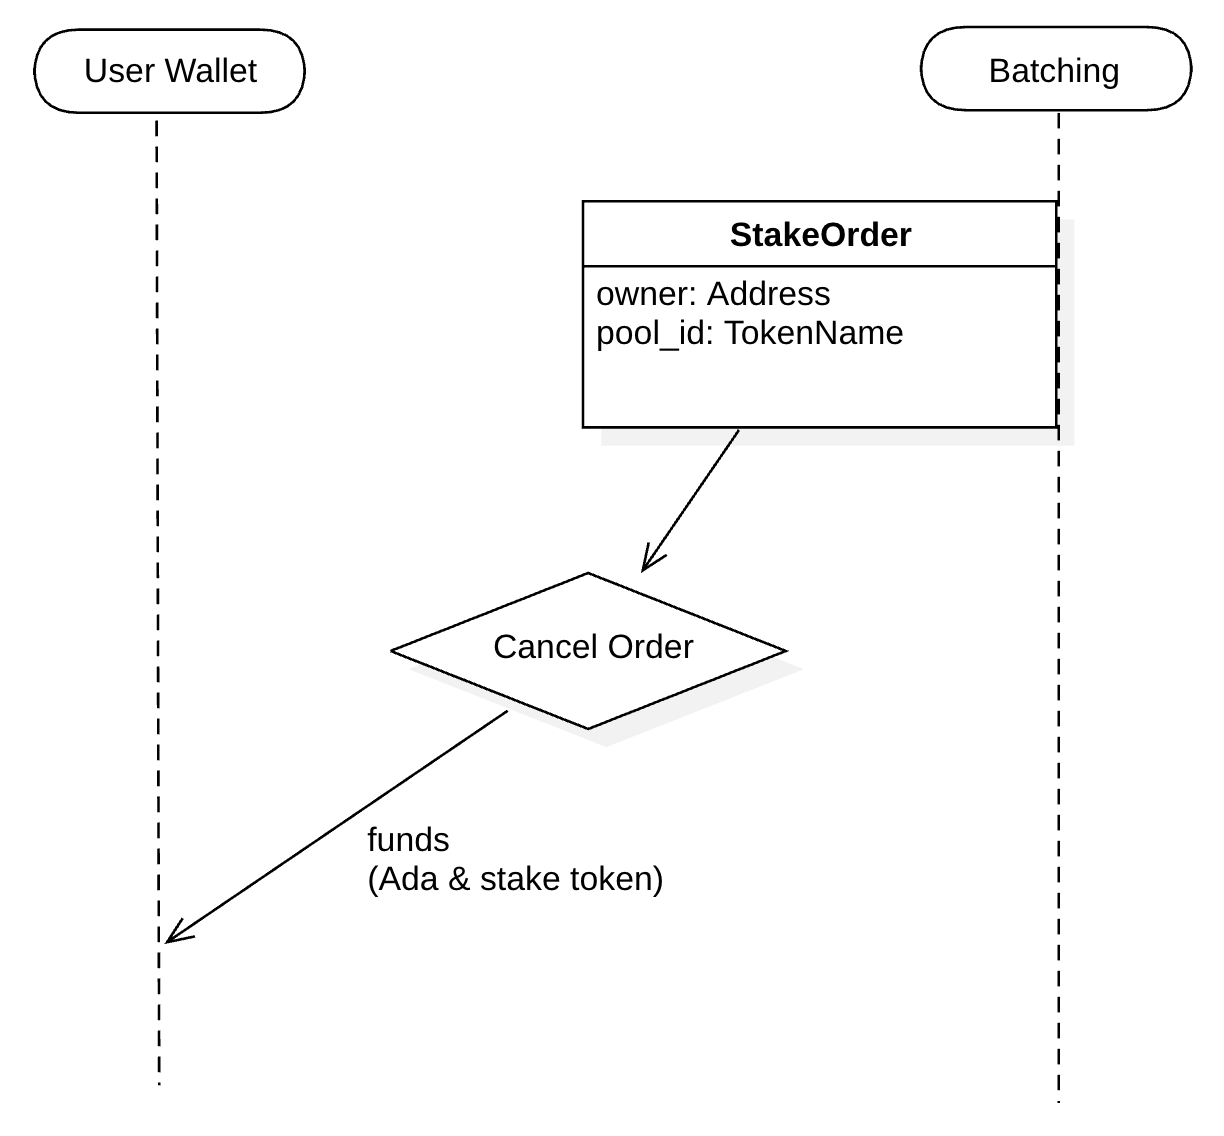
\includegraphics[width=\textwidth]{figures/cancel-stake-order.png}
        \caption{Cancelling a stake order.}
        \label{fig:cancel-stake-order}
    \end{subfigure}
\end{figure}

\textbf{Placing:} In a placing transaction (see Figure~\ref{fig:place-stake-order}), the user sends the tokens to be staked, along with some collateral Ada, to the Batching contract. This action creates a UTxO with a datum containing the owner's address and the pool\_id, representing the user's stake order.

\textbf{Cancelling:} Cancelling a stake order  (see Figure~\ref{fig:cancel-stake-order}) is as simple as spending the previously created order UTxO from the Batching contract. This requires the owner's signature (as specified in the datum) on the Cancel Order transaction.

\subsection{Farm Creation}

\begin{figure}
    \centering
    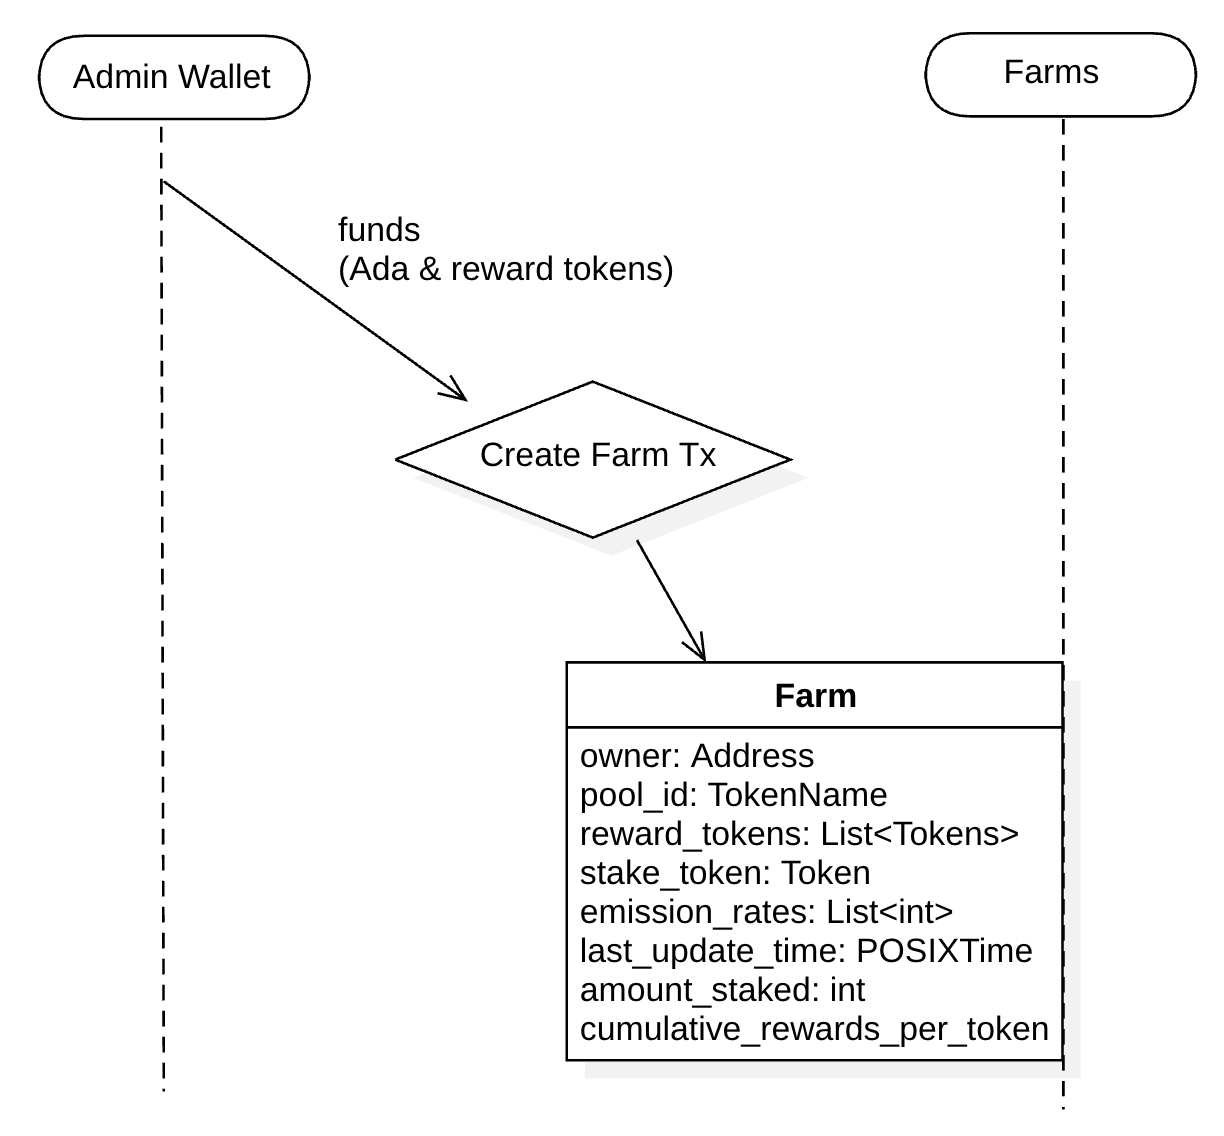
\includegraphics[width=.5\textwidth]{figures/create-farm-admin.png}
    \caption{Creating a farm (by an admin who provides the reward tokens).}
    \label{fig:create-farm-admin}
\end{figure}

A farm is created when a farm creator sends reward funds and some collateral Ada to the Farms contract. This action initializes a farm by creating a UTxO that includes the specified data fields related to the farm, as shown in the diagram in Figure~\ref{fig:create-farm-admin}.

\subsection{Batching of Stake Orders}

\begin{figure}
    \centering
    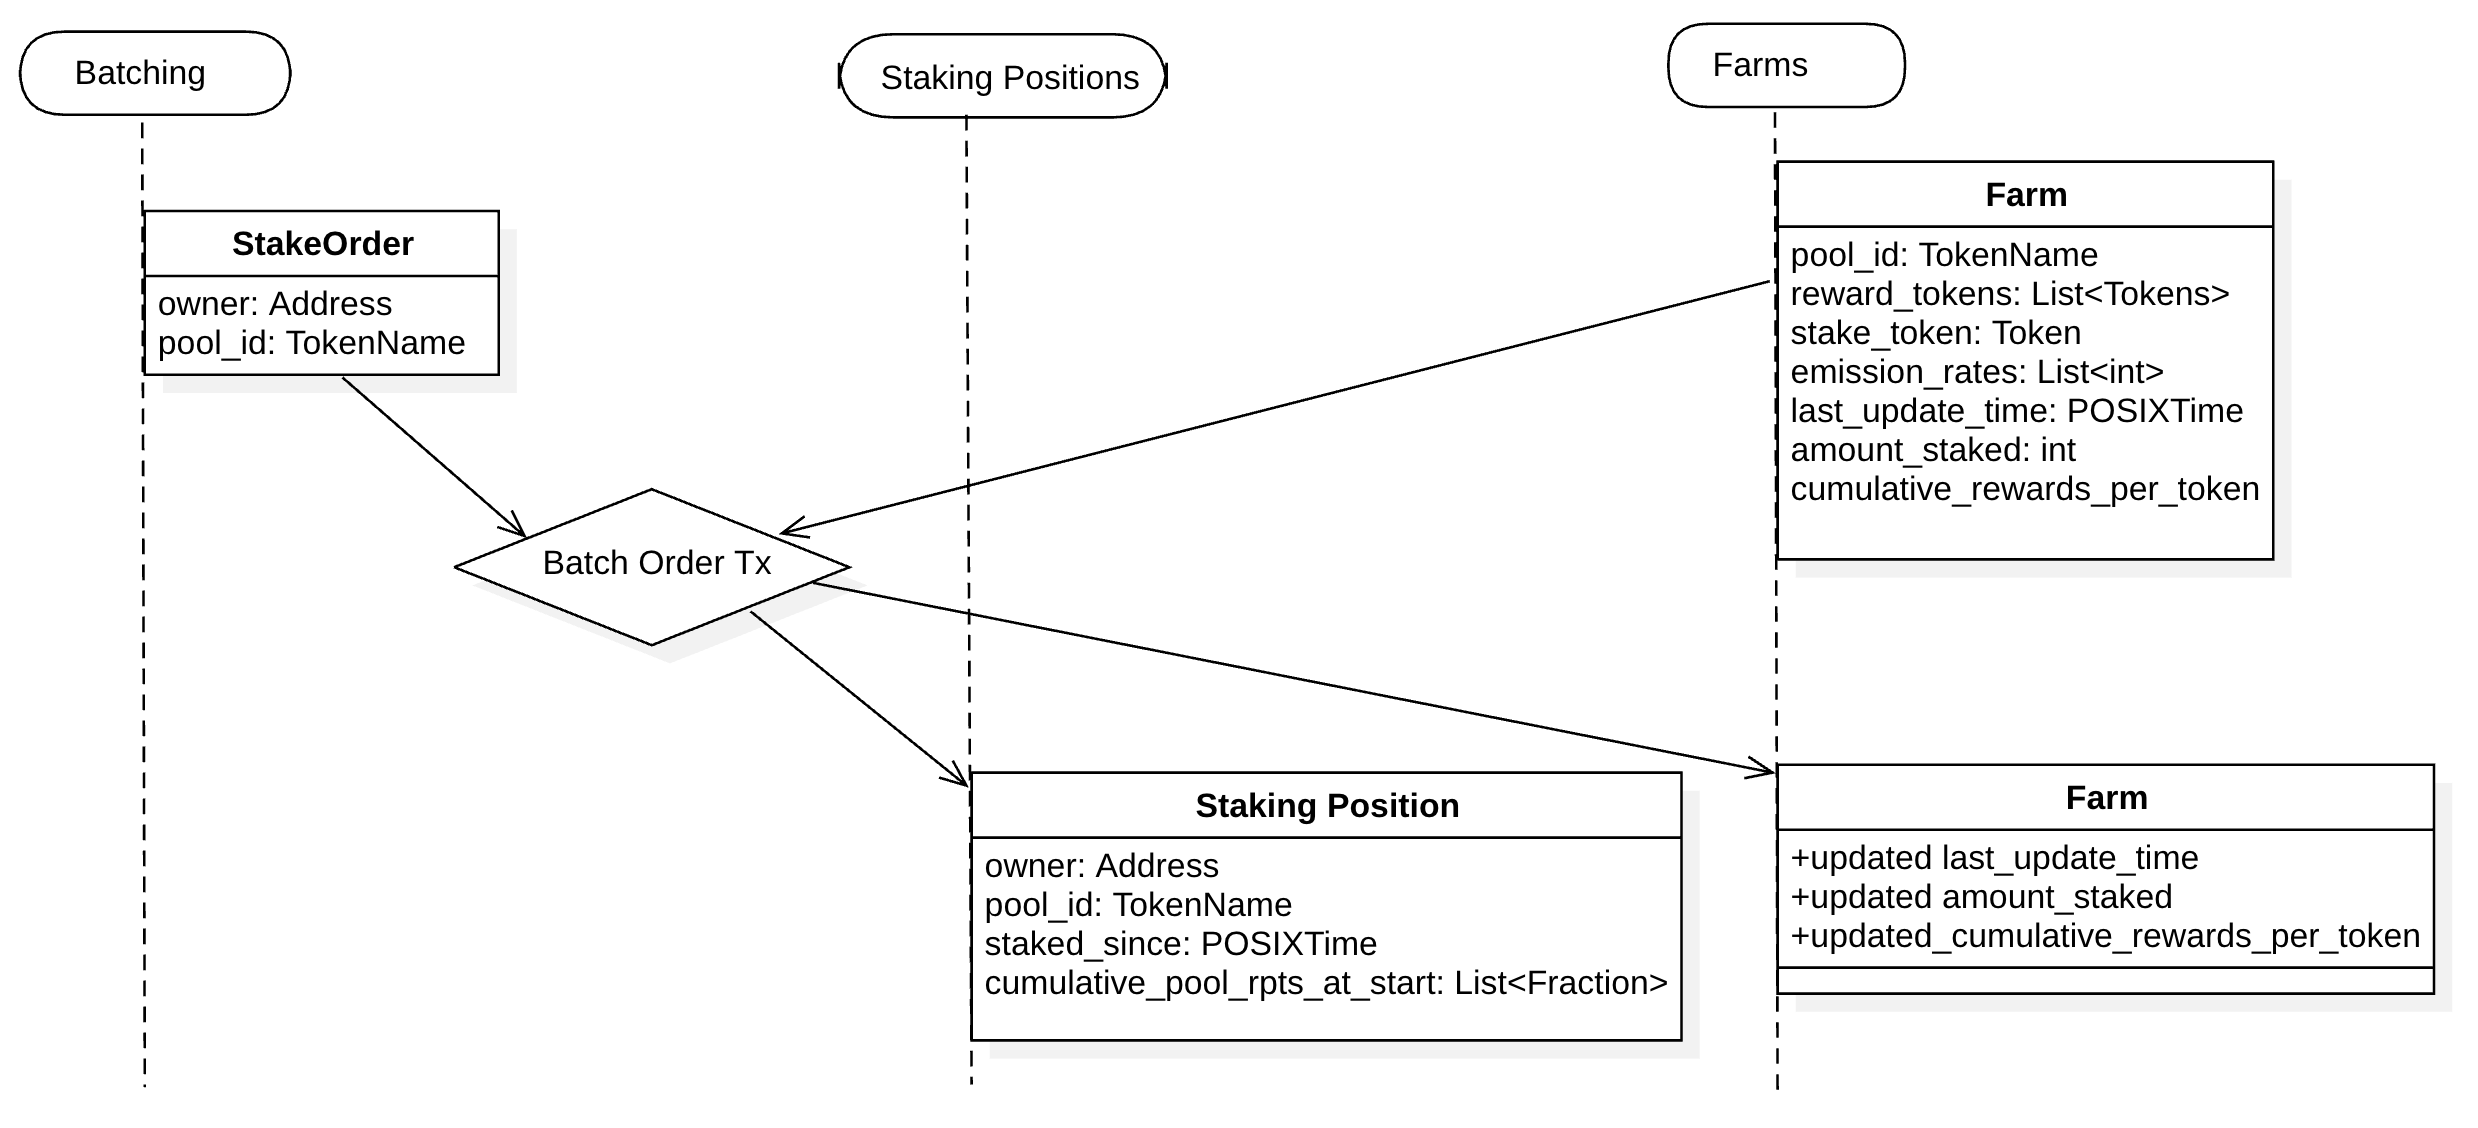
\includegraphics[width=\textwidth]{figures/batch-stake-order.png}
    \caption{Batching a stake order, i.e. gathering and updating the information from the farm by spending its UTxO and creating the Staking Position UTxO.}
    \label{fig:batch-stake-order}
\end{figure}

\textbf{Stake Order:} Represents a user's intention to stake tokens in a specific farm, containing details such as the owner's address, the pool ID, and the token being staked.

\textbf{Batch Order Transaction:} This transaction (see Figure~\ref{fig:batch-stake-order}) bundles multiple Stake Orders into one, executing the staking actions. Each Stake Order is processed, creating a corresponding Staking Position for the user.

\textbf{Staking Position:} This represents the user's staked tokens in the farm, including details like the owner, pool ID, staked amount, staking time, and cumulative rewards earned.

\subsection{Placing an Unstake Order}

\begin{figure}
    \centering
    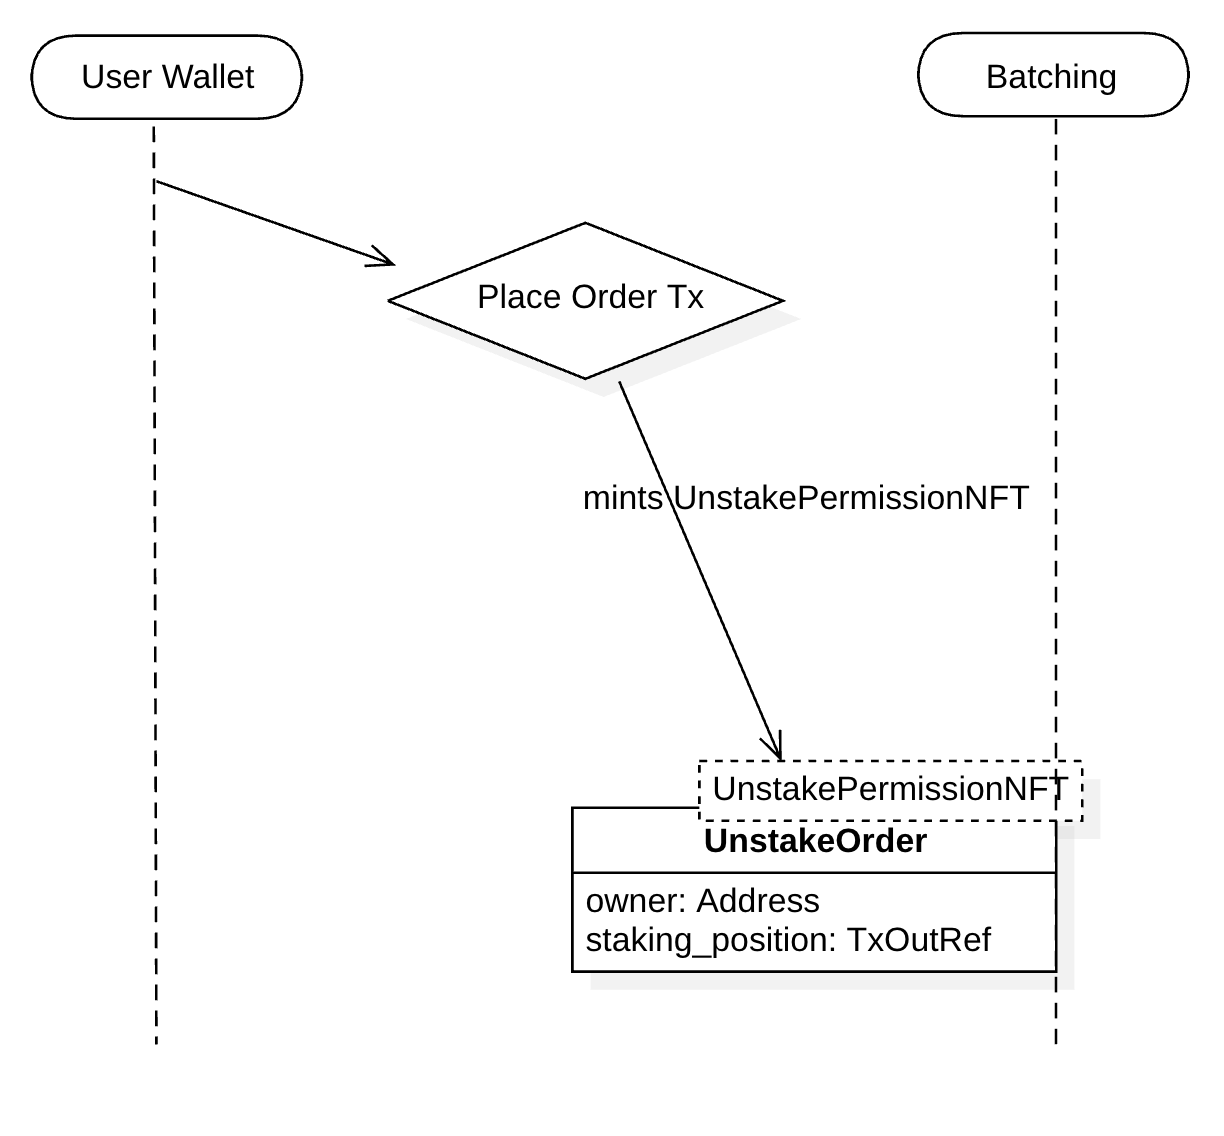
\includegraphics[width=.5\textwidth]{figures/place-unstake-order.png}
    \caption{Placing an unstake order by minting a respective UnstakePermissionNFT and locking it at the Batching contract.}
    \label{fig:place-unstake-order}
\end{figure}

Placing an unstake order (see Figure~\ref{fig:place-unstake-order}) is similar to placing a stake order, but it involves the minting of a permission NFT. This NFT grants a third-party batcher the authority to spend the UTxO created by a specific owner, ensuring that only authorized actions can unlock this UTxO.

\subsection{Batching an Unstake Order}

\begin{figure}
    \centering
    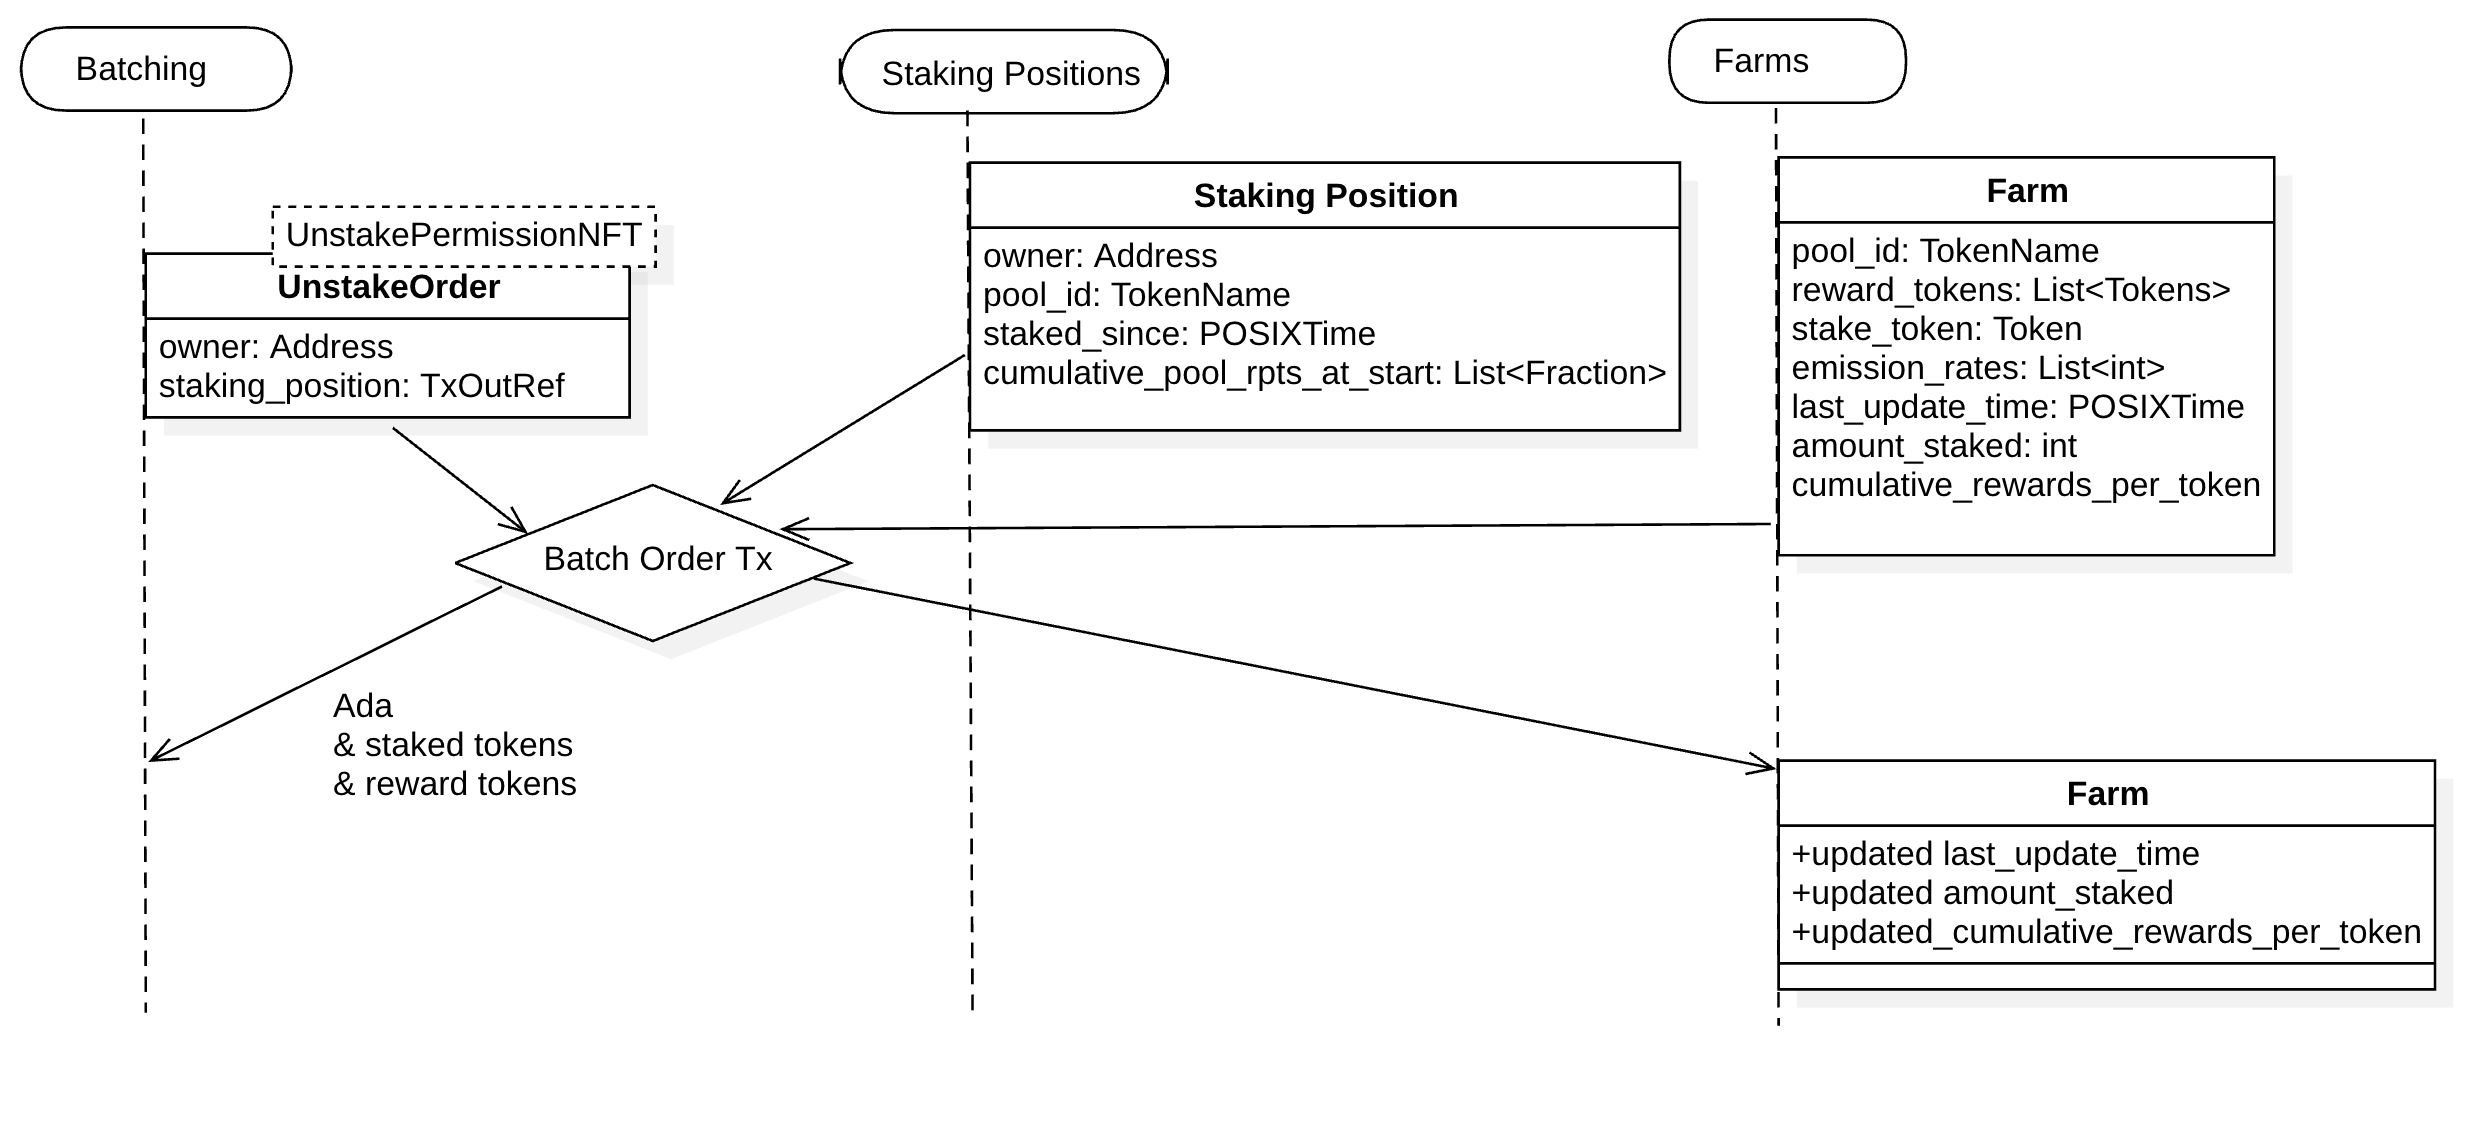
\includegraphics[width=\textwidth]{figures/batch-unstake-order.png}
    \caption{Batching an unstake order, i.e. gathering and updating the information from the farm by spending its UTxO and returning the tokens locked in the Staking Positions \& the respective rewards back to the user's wallet.}
    \label{fig:batch-unstake-order}
\end{figure}

Batching an unstake order (see Figure~\ref{fig:batch-unstake-order}) follows a process similar to batching a stake order. However, in this case, the staking position is used as input, and the staked funds along with the accrued rewards are paid out to the owner.


\section{Comparative Analysis of Existing Solutions}

In this section, we explore the current state of on-chain and off-chain staking and farming solutions on Cardano. Additionally, we investigate design choices in other blockchain ecosystems.

\subsection{Methodology}
This subsection outlines the methodology employed in the comparative analysis of existing staking and farming solutions. The primary goal of this analysis is to critically assess and compare various staking and farming models, highlighting their unique features, strengths, and limitations in the context of decentralized finance (DeFi) and incentive mechanisms.

\subsubsection{Selection Criteria for Staking and Farming Models}

Firstly, we collect all staking and farming models currently deployed or under development on the Cardano blockchain. Furthermore, we explore staking and farming models that are implemented on other blockchains based on their prevalence in the industry, innovativeness, impact on liquidity provision, and scalability.

\subsubsection{Data Collection and Sources}
Data and information regarding each staking and farming model are gathered from a variety of sources, including academic journals, press releases, reports, and whitepapers. This comprehensive approach ensures a well-rounded understanding of each model and its real-world implications.

\subsubsection{Evaluation Metrics}
The comparative analysis employs a set of predefined metrics to evaluate each staking and farming model. These metrics encompass:

\begin{itemize}
    \item \textbf{Decentralization:} Measuring the degree of power distribution among participants.
    \item \textbf{Efficiency:} Assessing the speed and resource utilization in reward distribution processes.
    \item \textbf{Security:} Evaluating the robustness of each model against common threats and vulnerabilities.
    \item \textbf{User Incentivization:} Analyzing how each model encourages and facilitates active participation from its stakeholders through rewards.
    \item \textbf{Interoperability:} Evaluating the ability of the solution to integrate and operate with other DeFi systems and blockchain platforms.
\end{itemize}

\subsubsection{Analytical Approach}
The analysis is conducted through a multi-dimensional approach, considering both qualitative and quantitative aspects of each model. Qualitative analysis provides insights into the staking and farming structures, user experience, and potential economic impacts. Quantitative analysis, on the other hand, involves statistical evaluation of performance metrics and user engagement data.

\subsubsection{Comparative Framework}
A structured comparative framework is employed to systematically evaluate each model against the set metrics. This framework aids in highlighting the contrasts and similarities among the various staking and farming models, providing a clear and concise comparative overview.

\subsubsection{Limitations and Assumptions}
The methodology acknowledges certain limitations and assumptions. Limitations may arise from the availability and recency of data, while assumptions are made regarding the general applicability of each model in different blockchain ecosystems. These factors are taken into account to ensure a balanced and fair analysis.

The outcome of this methodology is expected to provide valuable insights into the effectiveness and applicability of different staking and farming models, guiding future developments and decision-making processes in the realm of decentralized finance.


\subsection{Staking/Farming Solutions on Cardano}
Detailed analysis of existing staking/farming solutions on the Cardano platform.

\subsubsection{Current MuesliSwap Staking \& Farming System}

The MuesliSwap platform offers a staking and farming system where users can stake Cardano native tokens, unstake them, and receive additional reward tokens. Additionally, users have the option to harvest rewards without unstaking. In the context of farming, the system operates similarly, with the primary difference being that the staked tokens are LP (Liquidity Provider) tokens.

\paragraph{Staking Mechanism}

The staking model employed by MuesliSwap involves locking funds into a simple smart contract, with the owner's address recorded in the contract's datum. The system ensures security by only permitting unstaking transactions that have been signed by the owner, safeguarding the staked assets. Reward calculation and distribution are handled off-chain. Once a user decides to unstake or request a reward harvest, the rewards are sent in a separate transaction.

There are no lock-up periods associated with the basic staking mechanism on MuesliSwap. However, the platform also offers a Muesli-Vault system, which imposes a lock-up period by only allowing unstaking after a certain time slot, in addition to requiring the owner's signature.

\paragraph{Farming Mechanism}

MuesliSwap's farming mechanism is essentially an extension of the staking model, where users stake LP tokens instead of native tokens. The same smart contract and off-chain reward computation mechanisms apply. The rewards distributed through farming are periodically updated by the off-chain system maintainer.

\paragraph{Decentralization}

The MuesliSwap system operates in a semi-decentralized manner. The staking and locking processes are fully smart contract-based, which is crucial for the security of users' funds. However, the reward distribution process relies on a traditional centralized database that updates based on on-chain data, leaving room for further decentralization. Farming reward emissions are also adjusted centrally. For significant decisions regarding emissions, the MuesliSwap off-chain governance system is used, though the outcomes of these votes are not directly enforced on-chain.

\paragraph{Efficiency}

The reward distribution process on MuesliSwap is highly efficient, as it is based on a traditional database, which avoids the overhead associated with blockchain consensus mechanisms. The transaction costs are minimal because the smart contract's primary function is to verify the owner's signature without performing complex on-chain reward computations. This simplicity allows many unstaking transactions to fit within a single block, contributing to the system's scalability. Additionally, the separate reward distribution transactions can handle multiple payouts simultaneously within the same transaction, further enhancing scalability.

\paragraph{Security}

The security of users' staked assets on MuesliSwap is robust, with the simplicity of the smart contracts contributing to their safety. The straightforward nature of these contracts allows even non-technical users to understand how their funds are protected, which builds trust in the platform.

\paragraph{Interoperability}

MuesliSwap demonstrates a high degree of interoperability, particularly through its integration with Indigo Staking, which allows for reward payouts for staking positions on the Indigo platform. This integration was achieved by adding the necessary data to the centralized database, indicating that the system can easily accommodate interoperability with other platforms.


\subsubsection{Indigo Staking}

Indigo Protocol is a decentralized finance (DeFi) project on the Cardano blockchain, focusing on creating and managing synthetic assets, known as "iAssets." The Indigo staking mechanism serves multiple purposes, including governance, collateralization, earning rewards, and maintaining the peg of synthetic assets.

\paragraph{Staking Mechanism}

The Indigo staking mechanism is partially smart contract-based, similar to the MuesliSwap solution, but with additional complexity and functionality. Users can stake INDY tokens and adjust their stakes without the need to fully restake, thanks to the advanced features of the smart contracts. These contracts are also upgradable, allowing for the addition of new features and improvements over time. The source code for these smart contracts is publicly available and can be reviewed at the following link: \url{https://github.com/IndigoProtocol/indigo-smart-contracts/tree/main/src/Indigo/Contracts/Staking}.

However, despite the reliance on smart contracts, the computation and distribution of rewards remain centralized. Rewards are calculated off-chain, and the smart contracts do not enforce the validity of reward payouts. This means that, while the staking process itself is decentralized to some extent, the reward mechanism is under centralized control, which could be a potential point of concern for users seeking a fully decentralized solution.

The Indigo staking mechanism does not enforce strict minimum or maximum staking requirements, allowing flexibility for users. However, to mint iAssets, users must maintain a collateral ratio above a specified threshold to avoid liquidation. The protocol is designed to ensure that stakers maintain control over their staked assets, with no enforced lock-up periods for governance staking, although collateral used for minting iAssets is subject to liquidation risks if the value of the collateral falls too low.

\paragraph{Farming Mechanism}

While Indigo does not feature a traditional farming mechanism like those found in other DeFi protocols, the process of staking INDY tokens and providing liquidity to iAsset pools serves a similar purpose. Users can earn rewards for their participation in these activities, which helps incentivize the provision of liquidity and the stability of the synthetic assets within the Indigo ecosystem.

\paragraph{Decentralization}

Indigo Protocol aims to be decentralized, particularly in governance, where stakers of INDY tokens have significant influence. However, the level of decentralization is mixed. While the staking process itself is partially decentralized through the use of smart contracts, the reward distribution remains centralized, as it is managed off-chain and not enforced by the smart contracts.

The governance model allows stakers to vote on important decisions, such as protocol updates, new iAssets, and changes to collateralization processes. However, since the reward computation and payout are centralized, the overall decentralization of the protocol is limited. This centralization in the reward mechanism could reduce the influence of stakers on certain aspects of the protocol, particularly in ensuring transparency and trust in reward distributions.

\paragraph{Efficiency}

The reward distribution process in Indigo is managed efficiently, with rewards being allocated based on users' contributions to the protocol. The staking and collateral management processes are automated through smart contracts, ensuring that rewards are distributed without manual intervention. The Indigo Protocol is designed to be scalable, allowing it to handle increased user demand as the network grows. The use of smart contracts ensures that transaction costs remain low and that the system can process multiple staking and collateralization operations simultaneously.

The increased complexity of the smart contracts in Indigo also comes with higher execution costs. This makes the staking process more resource-intensive compared to simpler mechanisms like those used in MuesliSwap. The trade-off, however, is greater flexibility and functionality in managing stakes, which could appeal to more advanced users.

\paragraph{Security}

Indigo Protocol's staking mechanism is secured through the use of smart contracts on the Cardano blockchain. These contracts manage the staking process, collateralization, and reward distribution, ensuring that user funds are secure and that the protocol operates transparently. The protocol includes mechanisms to handle risks such as the devaluation of collateral, with liquidation processes in place to maintain stability. Indigo has not reported any major security breaches, but continuous updates and improvements are made to enhance the protocol's security.

\paragraph{User Incentivization}

Indigo incentivizes user participation through various reward programs. By staking INDY tokens or providing liquidity to iAsset pools, users can earn rewards in the form of additional INDY tokens or fees generated by the protocol. These rewards are designed to encourage active participation in the protocol's governance and the stability of synthetic assets. The reward structure is aligned to ensure fair distribution among participants, with additional incentives for those who contribute to the protocol's security and governance.

\paragraph{Interoperability}

Indigo Protocol is built on the Cardano blockchain and is designed to integrate with other DeFi platforms. The protocol's use of synthetic assets and collateralization mechanisms allows for potential interoperability with other blockchain networks and financial systems. However, the degree of interoperability may depend on the development of cross-chain compatibility features and the broader adoption of Indigo within the DeFi ecosystem.


\subsubsection{Comparison with Other DeFi Platforms}

Other DeFi platforms on Cardano, such as Minswap, SundaeSwap, and WingRiders, seem to employ similar techniques as those seen in Indigo and MuesliSwap, utilizing partially smart contract-based mechanisms for staking and farming. However, a significant limitation of these platforms is the lack of transparency in their operations. None of the smart contracts used by these platforms are open-source, and there is no detailed public documentation or audit available to verify what these contracts are actually doing.

This opacity makes it difficult for users to trust and fully evaluate the security, fairness, and efficiency of these platforms. The absence of transparency has led to growing demands within the Cardano DeFi community for a fully decentralized solution. Such a solution would be entirely smart contract-based, with open-source code and documentation of its functionality, setting a new standard for transparency, trust, and decentralization in the Cardano DeFi ecosystem.


\subsubsection{Cardano ADA Staking}

Last but not least: Cardano ADA staking is a core feature of the Cardano proof-of-stake (PoS) protocol, designed to secure the network and distribute rewards among participants who delegate their ADA to stake pools.

\paragraph{Important Note:} Cardano's built-in staking only concerns ADA, but no other native tokens. We include it here for completeness. However, it is clear that it does not meet the requirements of a staking or farming solution for use in DeFi platforms, as this necessarily requires support for any kind of native token.

\paragraph{Staking Mechanism}

Cardano utilizes a delegated proof-of-stake (dPoS) model, where ADA holders can delegate their tokens to a stake pool without transferring ownership. This delegation helps secure the network and participate in the block production process. Rewards are distributed automatically at the end of each epoch (a five-day period) based on the stake pool's performance, with delegators receiving a proportionate share of the rewards.

Cardano’s staking model is highly flexible, with no minimum or maximum staking requirements. ADA holders can delegate any amount of ADA to a stake pool, and there are no lock-up periods. Stakers retain full control over their funds, and they can redelegate or withdraw their staked ADA at any time.

\paragraph{Farming Mechanism}

Cardano ADA staking does not include a traditional farming mechanism as seen in DeFi protocols. Instead, the network rewards staking in a way that could be compared to yield farming, where users earn rewards based on their delegated stake. The primary asset involved is ADA, and the rewards are paid out in ADA, without the use of LP tokens or similar mechanisms.

\paragraph{Decentralization}

Cardano is designed with decentralization at its core. The staking mechanism supports this by enabling a large number of stake pools, each operated by independent entities or community groups. The protocol is governed by the community, with ADA holders influencing governance decisions through delegation. Over time, Cardano aims to further decentralize by gradually reducing the influence of the Cardano Foundation, IOHK, and Emurgo in network governance.

\paragraph{Efficiency}

The reward distribution process in Cardano is efficient and fully automated. Each epoch, the protocol calculates rewards based on the stake pool's performance and distributes them to delegators without requiring any manual intervention. The use of the Ouroboros protocol ensures that transaction costs remain low, and the system is highly scalable, capable of handling a growing number of transactions as the network expands.

\paragraph{Security}

Cardano’s PoS mechanism is underpinned by the Ouroboros protocol, which is formally verified and rigorously tested to ensure security. The staking mechanism itself is secure, with staked ADA remaining in the delegator's wallet, thus mitigating risks associated with fund transfer. Cardano has a strong track record with no major security breaches, and continuous updates and improvements are made to enhance the network's security.

\paragraph{User Incentivization}

Cardano incentivizes participation through staking rewards, which are distributed to both stake pool operators and delegators. The reward structure is designed to encourage decentralization by providing higher rewards to smaller, well-performing pools, thereby preventing centralization of stake.

\paragraph{Interoperability}

Cardano's interoperability efforts are ongoing, with future developments aimed at enhancing cross-chain compatibility. Currently, the network is working on integrating sidechains and enabling cross-chain transactions, which will further improve the staking mechanism's interoperability with other blockchain platforms.





\subsection{Staking/Farming Solutions on Other Platforms}
Next, we take a look outside the Cardano ecosystem. In particular, the focus here is on Ethereum DeFi protocols that include some staking mechnisms, as these platforms have existed the longest and hence seem the most matured.

\subsubsection{Aave Staking}

Aave is a major DeFi platform on Ethereum, offering a sophisticated staking mechanism through its Safety Module (SM). This module secures the protocol and provides rewards for participants.

\paragraph{General Overview}
The Aave Safety Module allows users to stake AAVE tokens and earn rewards while contributing to the protocol’s security. The staking mechanism is detailed in the
\href{https://github.com/aave/aave-stake-v2}{Aave Incentives contracts}, which outline how rewards are calculated and distributed. The staking contracts are partially decentralized, with smart contracts managing the staking process and reward distribution.

\paragraph{Staking Mechanism}
Aave’s staking mechanism involves several smart contracts:

\begin{itemize}
    \item \textbf{AaveDistributionManager:} This core contract manages the accounting for reward distributions. It calculates how many rewards are due to a user based on their stake and the duration of their participation. The contract handles multiple distributions, updates user states, and queries distribution information.
    \item \textbf{StakedAave:} This contract allows users to stake AAVE tokens and receive \texttt{stkAAVE} tokens in return. Users accrue rewards in AAVE, which can be claimed at any time. Withdrawals require a cooldown period to prevent rapid withdrawals.
    \item \textbf{AaveIncentivesController:} This contract manages incentives for activities on the Aave protocol. It updates rewards and handles reward claims through interactions with the Aave protocol.
\end{itemize}

The architecture and detailed specifications of these contracts are illustrated in Figure~\ref{fig:aave_staking_architecture}. The contracts handle both the staking and reward computation processes, ensuring that reward distribution is managed by the smart contracts but also involves off-chain components for some aspects of the reward calculation.

\begin{figure}[h!]
\centering
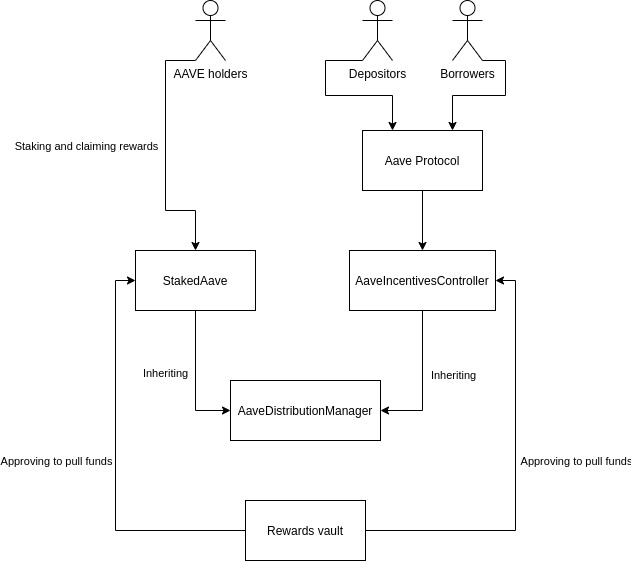
\includegraphics[width=0.8\textwidth]{figures/aave-stake-architecture}
\caption{Aave Staking Mechanism Overview}
\label{fig:aave_staking_architecture}
\end{figure}

\paragraph{Decentralization}
The Aave staking mechanism is decentralized through the use of smart contracts that enforce staking rules and reward distributions. The Aave protocol is governed by AAVE token holders, who participate in protocol decisions. While the smart contracts automate staking and reward distribution, some components, like reward computation, are managed off-chain, adding a layer of centralized control.

\paragraph{Efficiency}
The smart contracts for Aave staking are designed to be efficient, but their increased complexity can make them more expensive to execute compared to simpler contracts. The smart contracts support efficient reward distribution and scalability but involve a higher cost due to their sophisticated architecture and operations.

\paragraph{Security}
Aave’s staking mechanism benefits from Ethereum’s security and the robustness of its smart contracts. The contracts are subject to regular audits by organizations like Consensys Diligence and Certik, ensuring they are secure and reliable. You can review the code and audits on the \href{https://github.com/aave/aave-stake-v2}{Aave GitHub repository}.

\subsubsection{Sushi Swap \& Pancake Swap Staking/Farming}

Sushi Swap and Pancake Swap are leading decentralized exchanges that offer staking and farming solutions. Pancake Swap’s contracts are based on Sushi Swap's, making their mechanisms quite similar.

\paragraph{General Overview}
Both Sushi Swap and Pancake Swap provide staking and farming opportunities where users can earn rewards by providing liquidity or staking tokens. Their smart contracts manage these processes, ensuring a decentralized approach to reward distribution and liquidity management.

\paragraph{Staking/Farming Mechanism}
The staking and farming mechanisms on both platforms are implemented through smart contracts:

\begin{itemize}
    \item \textbf{Sushi Swap:} Utilizes the "MasterChef" contract to manage staking of LP tokens and distribute SUSHI rewards. The smart contracts handle reward calculations and distribution automatically.
    \item \textbf{Pancake Swap:} Employs a similar "MasterChef" contract to distribute CAKE rewards. The contracts are based on Sushi Swap's implementation but adapted for Pancake Swap's ecosystem.
\end{itemize}

The smart contracts for both platforms ensure that reward computations and distributions are handled in a decentralized manner. Users stake their LP tokens or other assets, and rewards are distributed according to the rules defined in the contracts.

\paragraph{Decentralization}
Both Sushi Swap and Pancake Swap use smart contracts to enforce staking and farming rules. This ensures a high level of decentralization, with reward computations and distributions managed by the contracts. The open-source nature of these contracts allows for community oversight and transparency.

\paragraph{Efficiency}
The smart contracts used by Sushi Swap and Pancake Swap are optimized for efficiency, minimizing transaction costs and handling high volumes of transactions effectively. Their design ensures that rewards are distributed promptly and accurately, supporting scalability as user participation grows.

\paragraph{Security}
The security of Sushi Swap and Pancake Swap is supported by their smart contracts and the underlying Ethereum and Binance Smart Chain blockchains. Regular audits and open-source code contribute to the security and trustworthiness of the platforms. You can review the smart contracts for each platform at the following links:
\begin{itemize}
    \item \href{https://github.com/Cori1109/sushiswap/tree/canary/contracts}{Sushi Swap smart contracts}
    \item \href{https://github.com/pancakeswap/pancake-smart-contracts/tree/master/projects/farms-pools/contracts}{Pancake Swap smart contracts}
\end{itemize}


\subsection{Best Practices and Lessons Learned}

This section summarizes the best practices identified and lessons learned from analyzing staking and farming solutions across not only Cardano, but also the Ethereum ecosystem.

We identify the following best practices:
\begin{enumerate}
    \item \textbf{Transparency and Open Source}
    Transparency is crucial for trust and security. Platforms should make their smart contracts open source and provide comprehensive documentation. This allows users to audit the code themselves and understand how the system operates. For example, Aave and Sushi Swap have embraced open-source practices, which enhance trust and facilitate community audits.

    \item \textbf{Decentralization of Core Functions}
    Decentralizing core functions, such as staking, governance, and reward distribution, helps in reducing the risk of central points of failure and enhances security. The trend in mature platforms shows a convergence toward increasingly decentralized solutions, as seen in "older" Ethereum-based platforms like Sushi Swap and Pancake Swap.

    \item \textbf{Flexibility and User Control}
    Providing flexibility in staking mechanisms, such as allowing users to withdraw or adjust their stakes without significant penalties, improves user experience. Platforms should avoid rigid lock-up periods unless necessary for specific use cases. Cardano’s staking model exemplifies this flexibility by allowing ADA holders to delegate their tokens without lock-up periods.

    \item \textbf{Continuous Improvement and Upgradeability}
    Continuous improvement is essential for adapting to evolving needs and mitigating new risks. Platforms should incorporate upgradeability into their smart contracts, ideally through a decentralized on-chain governance mechanism. This approach ensures that the protocol can evolve and address emerging challenges effectively. For instance, MuesliSwap is moving towards on-chain governance, which could be leveraged for on-chain staking and protocol upgradeability.

    \item \textbf{Efficient Reward Distribution}
    While efficiency in reward distribution is important, there is often a trade-off between efficiency and decentralization. Modern smart contract languages and technologies, like those used in OpShin, have minimized this concern by allowing for efficient yet decentralized solutions. Thus, efficiency in reward distribution no longer requires sacrificing decentralization.
\end{enumerate}

Moreover, as a conclusion from above, here are some of the most important lessons learned:
\begin{enumerate}
    \item \textbf{Complexity vs. Usability}
    Incorporating advanced features into staking mechanisms can add complexity, which might affect usability and transaction costs. Platforms should strive for a balance between sophisticated functionalities and ease of use. The increased complexity in Indigo Protocol’s staking mechanism introduces higher execution costs, which could be a barrier for less technical users.

    \item \textbf{Importance of Interoperability}
    Interoperability with other platforms and ecosystems can enhance the utility and attractiveness of a staking or farming solution. MuesliSwap’s integration with Indigo Staking illustrates the benefits of cross-platform compatibility. Platforms should consider how their solutions can interact with other DeFi projects and blockchain networks to maximize their impact.

    \item \textbf{Governance and Community Involvement}
    Active community involvement in governance helps in aligning the platform’s development with user needs and expectations. With MuesliSwap moving towards on-chain governance, there is an opportunity to leverage this for on-chain staking as well, including for the upgradeability of the protocol. Effective governance structures can drive innovation and ensure that the platform evolves in a way that benefits its users.

    \item \textbf{Managing Risks and Security}
    Security is a paramount concern in staking and farming solutions. Platforms must implement robust security measures and prepare for potential risks such as smart contract vulnerabilities and market fluctuations. Continuous monitoring and prompt responses to security threats are essential for maintaining user trust and safeguarding assets.

    \item \textbf{Scalability Considerations}
    Scalability is a critical factor for the long-term success of staking and farming platforms. Solutions should be designed to handle increasing transaction volumes and user participation without compromising performance. Efficient contract design and off-chain solutions, like those used by MuesliSwap, can help in managing scalability challenges effectively.
\end{enumerate}

In summary, adopting best practices such as transparency, decentralization, flexibility, and continuous improvement, while learning from challenges related to complexity, interoperability, and scalability, can significantly enhance the effectiveness and reliability of staking and farming solutions in the DeFi ecosystem.


% \subsection{Improvements Offered by Proposed System}
% \subsubsection{Enhanced Decentralization}
% Explanation of how the proposed system improves decentralization.

% \subsubsection{Improved Security}
% Description of security enhancements compared to existing solutions.

% \subsubsection{Efficiency and Scalability}
% Details on improvements in efficiency and scalability.

% \subsubsection{High Degree of Interoperability}
% Explanation of how the system achieves high interoperability with other platforms and solutions.


\section{Implementation Plan \& Development Phases}
This section outlines the breakdown of the development stages, tasks, and responsibilities required to implement the decentralized staking and farming system on Cardano. Each phase builds upon the previous one, ensuring a thorough and systematic development process.

\subsection{Research and Design}
The initial phase focuses on researching existing staking and farming solutions, both on Cardano and other blockchain platforms, and designing a comprehensive architecture for the proposed system. 

During this phase, the project team will:
\begin{itemize}
    \item Conduct an in-depth analysis of current decentralized staking systems, detailing their strengths and limitations.
    \item Develop a detailed architecture for a decentralized staking system, specifying the roles and interactions of the three main contract components: staking contracts, top-pools contracts, and governance-based farms.
    \item Compare the proposed system with existing solutions, highlighting improvements in decentralization and security.
    \item Document findings in a comprehensive report and publish a blog post outlining the research and implementation plan.
\end{itemize}

\subsection{On-Chain Component Development}
The second phase involves the actual development and implementation of the on-chain components of the system. This includes coding the staking contracts, top-pools contracts, and governance-based farms using the OpShin programming language.

Tasks in this phase include:
\begin{itemize}
    \item Implementing smart contracts for staking, top-pools, and governance-based farms.
    \item Conducting an internal security audit to ensure the robustness and security of the code.
    \item Deploying the on-chain components in a controlled environment for initial testing.
    \item Publishing a detailed blog post on the on-chain implementation and audit results.
\end{itemize}

\subsection{Off-Chain Infrastructure Development}
The third phase focuses on developing the off-chain infrastructure necessary to manage and interact with the on-chain components. This off-chain code will facilitate transactions, manage staking contracts, and maintain top-pools and governance-based farms.

Key activities include:
\begin{itemize}
    \item Developing off-chain code to handle interactions with the staking contracts, top-pools contracts, and governance-based farms.
    \item Testing the integration of off-chain and on-chain components using testnet transactions.
    \item Documenting the successful interplay between off-chain infrastructure and on-chain code through detailed testnet results.
    \item Summarizing the testing phase and outcomes in a comprehensive report.
\end{itemize}

\subsection{Deployment, User Feedback Integration, Finalization, and Release}
The final phase involves deploying the alpha version of the system, collecting user feedback, making necessary adjustments, and launching the fully implemented system on MuesliSwap.

Tasks in this phase include:
\begin{itemize}
    \item Deploying an alpha version of the system to collect user feedback.
    \item Implementing adjustments based on feedback from internal audits and the community.
    \item Officially launching the fully implemented farming system on MuesliSwap.
    \item Publishing a final close-out report and a video detailing the deployment and finalization process.
\end{itemize}

By following these structured development phases, the project ensures a comprehensive and systematic approach to building a secure, decentralized, and user-friendly staking and farming solution on Cardano.


\section{Conclusion}
In conclusion, the proposed decentralized farming and staking system for Cardano represents a significant advancement in achieving full decentralization. By leveraging modern smart contract techniques and languages, the system ensures that all components, including reward computation, operate entirely on-chain. This approach not only enhances trust and security but also sets a new standard for transparency and community governance in decentralized finance. The comparative analysis of existing solutions highlights the need for such advancements, emphasizing the importance of complete decentralization in fostering a more resilient and user-centric DeFi ecosystem. The outlined implementation plan provides a clear path towards realizing this vision, promising a robust and innovative solution for the Cardano community.


\end{document}
